\chapter{GIRAF Outline}

The project we worked on this semester was the \gls{giraf} project. The following section describes what the project is, as well as the state at handover.

People with an \gls{asd} can have difficulties with communication. \gls{giraf} is a tablet environment developed to ease communication between people with an \gls{asd} and the people who take care of them. In this report we refer to them as \glspl{citizen} and \glspl{guardian} respectively.

Some software students from Aalborg University develop \gls{giraf} for their bachelor project. These students work in small teams and coordinate the work between teams. The students collaborate with the following institutions \cite{GirafWebsite}, who act as customers in the development process.

\begin{itemize}
    \item Børnehaven Birken (Kindergarten) \cite{bhBirken}
    \item Egebakken (School) \cite{egebakken}
    \item Enterne (Home for disabled) \cite{enterne}
    \item The speech institute at Aalborg municipality
    \item Center for Autism and ADHD \cite{center_for_autism}
\end{itemize}

The project started in 2011, and each year, the students continue where the previous year's students left off. 

We started this semester, like previous years have, by deciding to use the \gls{Scrum_principles}. One team got assigned the role of the \gls{PO}  while another got assigned the role of \gls{SMT}. The \gls{PO} team is responsible for the product backlog and customer communication. The \gls{SMT} decides how the process is defined, and make guidelines for the \glspl{devTeam}.

\section{The Current state of GIRAF}

The \gls{giraf} project has had multiple applications under its belt, which all shared the same backend. In 2017 the \glspl{devTeam} decided to upgrade the backend and disregard backward-compatibility \cite{SW608F18}, which left all existing applications unusable. All except one, the Weekplanner, which, fortunately, the glspl{devTeam} had rebuilt to be compatible with the upgraded backend.

Since 2017, of all the applications in the \gls{giraf} project, only the Weekplanner has been updated, and as such, is the only application of any interest to the customers. We decided to limit our development to the Weekplanner. 

The backend is a .NET Core 2 project that uses traditional MVC and supports all the capabilities of the current Weekplanner app. It exposes a REST-inspired API. \autoref{fig:RestAPIFigure} shows how the Weekplanner application can communicate with the backend.

\begin{figure}[H]
        \begin{center}
            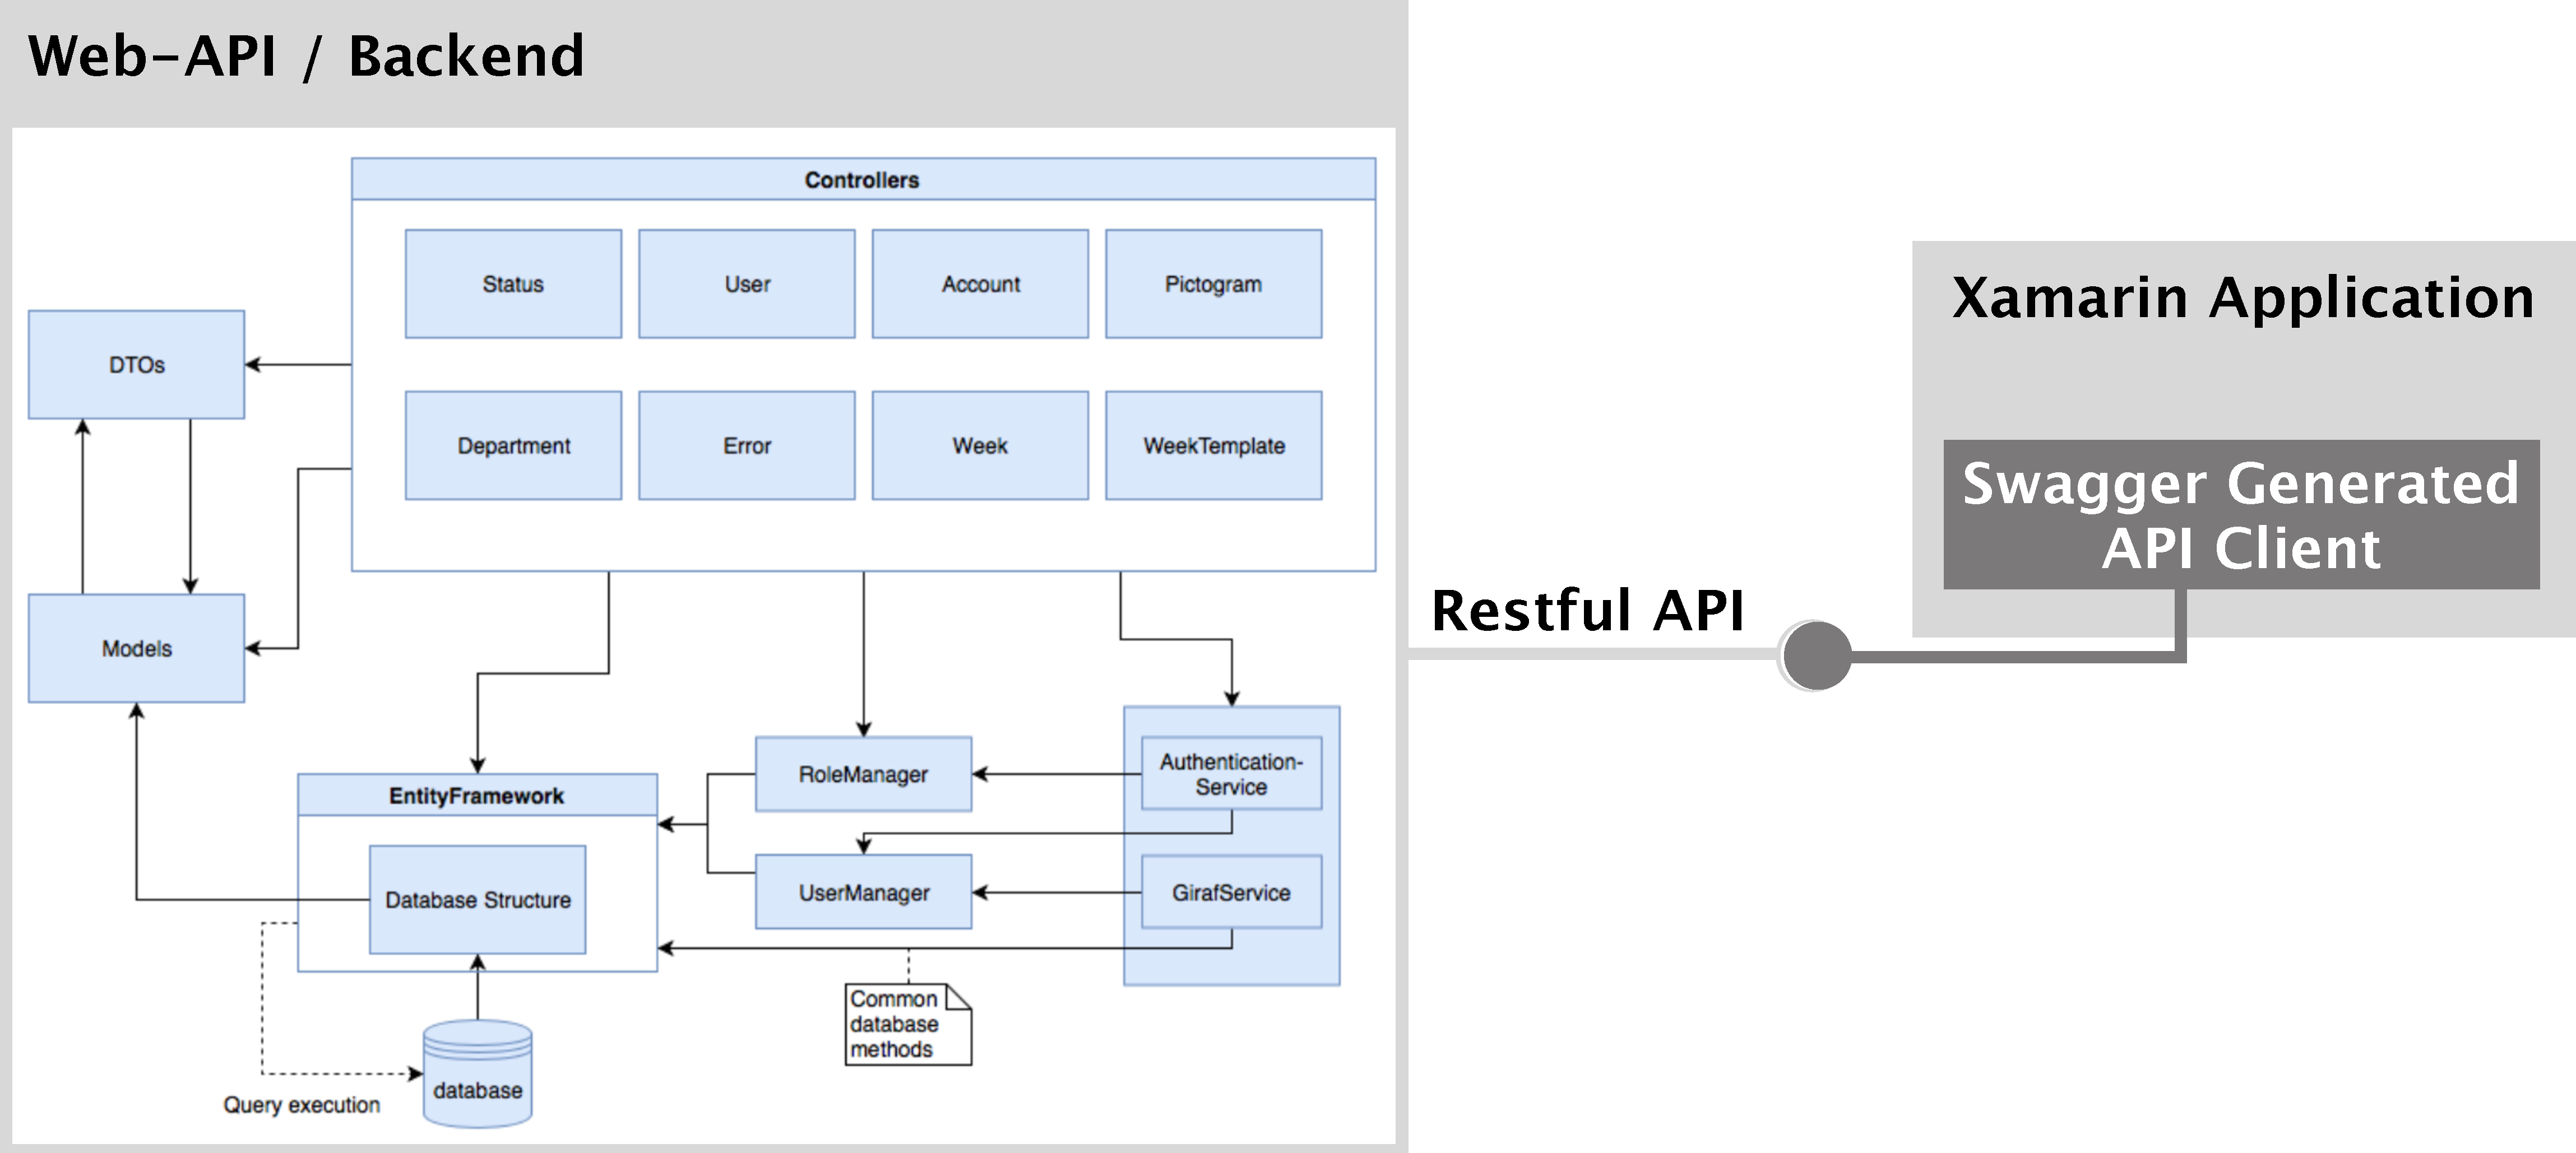
\includegraphics[width=0.95\textwidth]{figures/RestAPIFigure.pdf}
        \end{center}
        \caption{Illustration of the .NET Core 2 project and how it exposes a RESTful API}
        \label{fig:RestAPIFigure}
\end{figure}

